\documentclass[addpoints,12pt]{exam}
\usepackage[spanish]{babel}
%\usepackage[latin1]{inputenc}
\usepackage[utf8x]{inputenc}
\usepackage{graphicx}
\pagestyle{empty}
\begin{document}
\begin{center}
\fbox{\fbox{\parbox{5.5in}{\centering {\LARGE EXAMEN TIPO A}\\Sigue las intrucciones que marca el ejercicio, no solo para la realización del mismo sino también para la entrega.\\\emph{No se permite ningun documento de ayuda, excepto los aportados por el profesor}\\Se permite la realización del ejercicio en Eclipse o Netbeans utilizando un workspace vacío y crea un \emph{package} denominado \emph{\textit{segundaevaluacion}}}}}
\end{center}
\vspace{0.1in}
%\makebox[\textwidth]{Nombre:\enspace\hrulefill}

\begin{questions}

\question Crea una clase denominada \emph{Ejercicio1} que incorpore la librería externa \emph{auxiliar.jar}. Crea dos objetos de tipo \emph{Numero} y comprueba el funcionamiento de todos los métodos que contiene dicha clase \emph{Numero} en el diagrama UML.
\\
Posteriormente crea un jar ejecutable denominado \emph{ejercicio1.jar}\\
\vspace{0.3cm}
\\
Criterios de evaluación:
\begin{description}
\item[1 pto.] Funcionamiento correcto de la clase \emph{Ejercicio1}.
\item[1 pto.] Funcionamiento correcto de la clase \emph{ejercicio1.jar}.
\end{description}
En el caso que no seas capaz de incorporar dicha biblioteca, puedes diseñar la parte que te corresponde en una clase aparte y posteriormente realizar el ejercicio tal y como se te pide. En este caso la puntuación del ejercicio es de solo 1 punto y siempre y cuando esté funcionando correctamente. 
\begin{figure}[h]
\centering
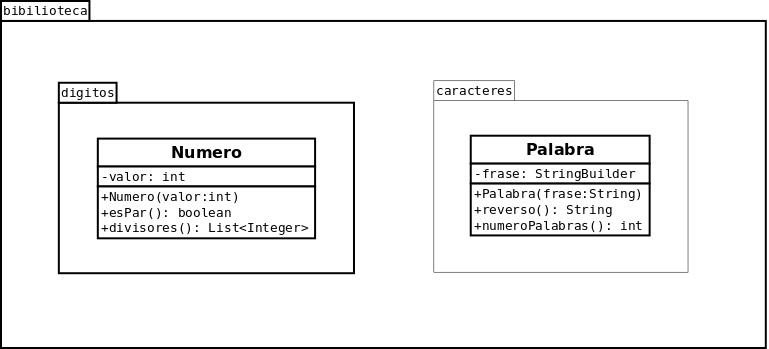
\includegraphics[scale=0.3]{examen.png}
\caption{Diagrama UML para el ejercicio 1}
\end{figure}
\question Crea una clase denominada \emph{Ejercicio2} que cree una lista de tipo \emph{ArrayList} de objetos de tipo \emph{Persona}. Para la creación de objetos de tipo \emph{Persona} usarás un \emph{Scanner} que lea los atributos y añadirá a la lista siempre y cuando dicho objeto sea válido de acuerdo al método \emph{esValido()} en cuál dará como aceptable a un objeto \emph{Persona} siempre y cuando los atributos \emph{nombre y apellido1} no sean cadenas vacías, el atributo \emph{telefono} contenga seis dígito y comience bien por 6 o por 9 y el \emph{email} contiene la @.\\
Posteriormente imprimiras por pantalla los valores que contiene la lista. \\
También deberás recorrer la lista de objetos \emph{Persona} y extraerás el atributo \emph{email} de la misma y lo añadirás a un \emph{StringBuilder} usando como separador de campos un guión. Ejemplo: \emph{emmm@jkfjdk.es-fjdj@fjfj.com-qrr@jfkd.it-bbcu@fh.de}, observa que el último campo no tiene separador. \\
Para esta última parte puedes añadir a la clase \emph{Persona} algún \emph{getter} que pudiera hacerte falta.\\
Para comprobar el correcto funcionamiento de esta última parte muestra por pantalla dicho \emph{StringBuilder}\\
Para acabar el \emph{Scanner} usa la palabra \emph{quit} cuando intentes leer el atributo \emph{nombre}.\\
También crearás un jar ejecutable denominado \emph{ejercicio2.jar} así como la documentación en \emph{javadoc} de la clase \emph{Persona}. Esta debe aparecer en el \emph{workspace}
\vspace{0.3cm}
\\
Criterios de evaluación:
\begin{description}
\item[2 ptos.] Funcionamiento correcto de la clase \emph{Persona}.
\item[1 pto.] Funcionamiento correcto del clase \emph{Scanner}.
\item[0.5 ptos.] Creación correcta de la lista.
\item[1.5 ptos.] Creación del StringBuilder.
\item[0.5 ptos.] Creación del jar ejecutable.
\item[0.5 ptos.] Creación de la documentación. 
\end{description}
\begin{figure}[h]
\centering
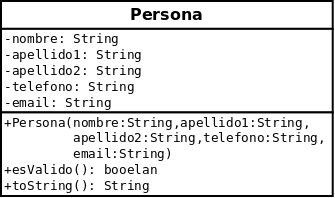
\includegraphics[scale=0.5]{persona.png}
\caption{Diagrama UML para el ejercicio 2}
\end{figure}
\end{questions}
%\newpage
\textbf{Formato del fichero de subida:} se subirá un archivo comprimido de la siguiente forma nombreApellidos.tar.gz o nombre.Apellidos.zip. En el debes incluir:
\begin{itemize}
\item El \emph{workspace} donde has realizado el examen. 
\item El fichero jar ejecutable del primer ejercicio.
\item El fichero jar ejecutable del segundo ejercicio.
\end{itemize}


\end{document}
